\documentclass[9pt,c]{beamer} 
\usepackage[utf8]{inputenc}
\usepackage[T1]{fontenc}
\fontfamily{ppl}\selectfont

\usepackage{fontspec} 
\defaultfontfeatures{Mapping=tex-text} 
\setsansfont[Ligatures={Common}]{Futura}
\setmonofont[Scale=0.8]{Monaco} 



%\setbeamersize{text margin left=10pt,text margin right=10pt}
\usetheme{lehigh}

\usefonttheme{professionalfonts}
\usefonttheme{serif}

\pgfdeclarelayer{background}
\pgfdeclarelayer{foreground}
\pgfsetlayers{background,main,foreground}

% add packages to use
%\usepackage[latin1]{inputenc}
%\usepackage[english]{babel}
%\usepackage[normalem]{ulem}
\usepackage{times}
\usepackage[T1]{fontenc}
\usepackage{pgf,pgfarrows,pgfnodes,pgfautomata,pgfheaps,pgfshade}
\usepackage{amsmath,amssymb,amsfonts,subfigure,pifont}
\usepackage{graphicx}
\usepackage{multirow,multicol}
\usepackage{tabularx}
\usepackage{booktabs}
\usepackage{colortbl}
\usepackage{fancyvrb,listings}
\usepackage{algorithm,algpseudocode}
%\usepackage{keystroke}
\usepackage{etex}
\usepackage{hyperref}
\usepackage{tikz}
\usetikzlibrary{trees,matrix,shapes,arrows}
\usetikzlibrary{calc}



% The following color are for listing environment 
\definecolor{dkgreen}{rgb}{0,0.6,0}
\definecolor{DarkGreen}{rgb}{0.0,0.3,0.0}
\definecolor{gray}{rgb}{0.5,0.5,0.5}
\definecolor{mauve}{rgb}{0.58,0,0.82}
\definecolor{Blue}{rgb}{0.0,0.0,0.8} 
\definecolor{dodgerblue}{rgb}{0.1,0.1,1.0}
\definecolor{indigo}{rgb}{0.41,0.1,0.0}
\definecolor{seagreen}{rgb}{0.1,1.0,0.1}


\lstset{%
language=bash,                % the language of the code
basicstyle=\tiny\ttfamily,           % the size of the fonts that are used for the code
showspaces=false,               % show spaces adding particular underscores
showstringspaces=false,         % underline spaces within strings
showtabs=false,                 % show tabs within strings adding particular underscores
%frame=single,                   % adds a frame around the code
%rulecolor=\color{black},        % if not set, the frame-color may be changed on line-breaks within not-black text (e.g. comments (green here))
tabsize=2,                      % sets default tabsize to 2 spaces
%captionpos=b,                   % sets the caption-position to bottom
breaklines=true,                % sets automatic line breaking
breakatwhitespace=false,        % sets if automatic breaks should only happen at whitespace
%title=\lstname,                   % show the filename of files included with \lstinputlisting;
% also try caption instead of title
keywordstyle=\color{blue},          % keyword style
commentstyle=\color{dkgreen},       % comment style
stringstyle=\color{mauve},         % string literal style
escapeinside={!}{!},            % if you want to add LaTeX within your code
morekeywords={*,\dots,elif},              % if you want to add more keywords to the set
deletekeywords={\dots},              % if you want to delete keywords from the given language
%morecomment=[l]{//}
}
\lstset{%
language=csh,                % the language of the code
basicstyle=\tiny\ttfamily,           % the size of the fonts that are used for the code
showspaces=false,               % show spaces adding particular underscores
showstringspaces=false,         % underline spaces within strings
showtabs=false,                 % show tabs within strings adding particular underscores
%frame=single,                   % adds a frame around the code
%rulecolor=\color{black},        % if not set, the frame-color may be changed on line-breaks within not-black text (e.g. comments (green here))
tabsize=2,                      % sets default tabsize to 2 spaces
captionpos=b,                   % sets the caption-position to bottom
breaklines=true,                % sets automatic line breaking
breakatwhitespace=false,        % sets if automatic breaks should only happen at whitespace
%title=\lstname,                   % show the filename of files included with \lstinputlisting;
% also try caption instead of title
keywordstyle=\color{blue},          % keyword style
commentstyle=\color{dkgreen},       % comment style
stringstyle=\color{mauve},         % string literal style
escapeinside={\%*}{*)},            % if you want to add LaTeX within your code
morekeywords={*,\dots,elif},              % if you want to add more keywords to the set
deletekeywords={\dots},              % if you want to delete keywords from the given language
%morecomment=[l]{//}
}

\lstdefinestyle{LINUX}
{
    backgroundcolor=\color{white},
    basicstyle=\tiny\ttfamily,
    keywordstyle=\color{blue},
    morekeywords={apacheco,Tutorials,BASH,scripts,day1,examples},
    literate={>}{{\textcolor{blue}{>}}}1
         {/}{{\textcolor{blue}{/}}}1
         {./}{{\textcolor{black}{./ }}}1
         {~}{{\textcolor{blue}{\textasciitilde}}}1,
}

\lstdefinestyle{customc}{
  belowcaptionskip=1\baselineskip,
  breaklines=true,
  xleftmargin=\parindent,
  language=C,
  showstringspaces=false,
  basicstyle=\tiny\ttfamily,
  keywordstyle=\bfseries\color{green!40!black},
  commentstyle=\upshape\color{red!90!white},
  identifierstyle=\color{blue},
  stringstyle=\color{orange},
}
\lstdefinelanguage{OmpFortran}[]{Fortran}{
   rulesepcolor=\color{black},
   %
   extendedchars=true,
   %
   morecomment=[l] [\bfseries\color{red!90!white}]{!\$omp},
   morecomment=[l] [\bfseries\color{red!90!white}]{c\$omp},
   morecomment=[l] [\bfseries\color{red!90!white}]{*\$omp},
   morecomment=[l] [\bfseries\color{red!90!white}]{!\$acc},
   morecomment=[l] [\bfseries\color{red!90!white}]{c\$acc},
   morecomment=[l] [\bfseries\color{red!90!white}]{*\$acc},
}[comments]

\lstdefinelanguage{OmpC}[]{OmpFortran}{
   rulesepcolor=\color{black},
   %
   extendedchars=true,
   %
   morecomment=[l] [\bfseries\color{red!90!white}]{\#pragma\ omp},
   morecomment=[l] [\bfseries\color{red!90!white}]{\#pragma\ acc},
}[comments]

\lstset{escapechar=@,style=customc}
\lstset{literate=%
   *{0}{{{\color{blue}0}}}1
    {1}{{{\color{blue}1}}}1
    {2}{{{\color{blue}2}}}1
    {3}{{{\color{blue}3}}}1
    {4}{{{\color{blue}4}}}1
    {5}{{{\color{blue}5}}}1
    {6}{{{\color{blue}6}}}1
    {7}{{{\color{blue}7}}}1
    {8}{{{\color{blue}8}}}1
    {9}{{{\color{blue}9}}}1
}

\algrenewcommand\algorithmicfunction{\textbf{program}}
\algblockdefx[Program]{Program}{EndProgram}[1]{\textbf{program} \textsc{#1}}[1]{\textbf{end program} \textsc{#1}}
\algloopdefx[doloop]{Do}[1]{\textbf{do} #1}
\algcblockdefx[doloop]{If}{Do}{EndDo}
[1]{\textbf{do} #1}{\textbf{end do}}


\DeclareSymbolFont{extraup}{U}{zavm}{m}{n}
%\DeclareMathSymbol{\vardiamond}{\mathalpha}{extraup}{87}
\newcommand{\cmark}{\ding{51}}
\newcommand{\xmark}{\ding{55}}
\newcommand{\smark}{\ding{77}}
\newcommand*\vardiamond{\textcolor{lubrown}{%
  \ensuremath{\blacklozenge}}}
\newcommand*\mybigstar{\textcolor{lubrown!90!yellow}{%
  \ensuremath{\bigstar}}}
\newcommand*\up{\textcolor{green!80!black}{%
  \ensuremath{\blacktriangle}}}
\newcommand*\down{\textcolor{red}{%
  \ensuremath{\blacktriangledown}}}
\newcommand*\const{\textcolor{darkgray}%
  {\textbf{--}}}
\newcommand*\enter{\tikz[baseline=-0.5ex] \draw[<-] (0,0) -| (0.5,0.1);}
\newcommand{\bftt}[1]{\textbf{\texttt{#1}}}
\newcommand{\bflub}[1]{\textbf{\color{lubrown}#1}}
\newcommand{\lstfortran}[1]{\lstinline[language={[90]Fortran},basicstyle=\small\ttfamily]|#1|}
\newcommand{\lstC}[1]{\lstinline[language=C,basicstyle=\small\ttfamily]|#1|}
\newcommand{\Verblubrown}[1]{\Verb[formatcom=\color{lubrown},fontseries=b,commandchars=\\\{\}]|#1|}
\newcommand{\Verblue}[1]{\Verb[formatcom=\color{lublue},fontseries=b,commandchars=\\\{\}]!#1!}
\newcommand{\Verbblue}[2][b]{\Verb[formatcom=\color{lublue},fontshape=#1,commandchars=\\\{\}]|#2|}
\newcommand{\Verblubrownp}[1]{\Verb[formatcom=\color{lubrown},fontseries=b,commandchars=\\\{\}]!#1!}
\newcommand{\Verbred}[1]{\Verb[formatcom=\color{red},commandchars=\\\{\}]|#1|}
\newcommand{\Verbindigo}[1]{\Verb[formatcom=\color{indigo},fontsize=\fontsize{7.5}{8}\selectfont,commandchars=\\\{\}]!#1!}

\newcolumntype{a}{>{\columncolor{lulime}}c}
\newcolumntype{b}{>{\columncolor{lulime!50}}c}
\newcolumntype{d}{>{\columncolor{lulime!40}}c}
\newcolumntype{e}{>{\columncolor{lulime}}l}
\newcolumntype{f}{>{\columncolor{lulime!50}}l}

                           
% LOGOS
\pgfdeclareimage[height=0.55cm]{lucolor-logo}{LehighU_official-logo_Color.png}
\rplogo{\pgfuseimage{lucolor-logo}}
\pgfdeclareimage[height=0.55cm]{luwhite-logo}{LehighU_official-logo_White.png}
\tplogo{\pgfuseimage{luwhite-logo}}
% footer logo
%\pgfdeclareimage[width=0.3\paperwidth]{university-logo}{lulogo}
%\tllogo{\pgfuseimage{university-logo}}

%titlepage logo
%\titlegraphic{
\includegraphics[scale=0.5]{lu}}

\beamertemplateballitem



\title[MPI]{Introduction to MPI}
\subtitle{HPC~Workshop:~Parallel~Programming}
\author{\large{Alexander~B.~Pacheco}}
\institute[Lehigh University Research Computing]{\href{http://researchcomputing.lehigh.edu}{Research~Computing}}
\date{}%July~13~-~15,~2021}
    
\AtBeginSection[]
{
  \begingroup
%  \setbeamertemplate{background canvas}[vertical shading][bottom=lubrown,top=lubrown]
%  \setbeamertemplate{footline}[myfootline] 
%  \setbeamertemplate{section page}[mysection]
  \frame[c]{
%    \sectionpage
    \tableofcontents[currentsection,currentsubsection]
  }
  \endgroup
}

\begin{document}

\begin{frame}
  \titlepage
\end{frame}

\begin{frame}
  \frametitle{Distributed Memory Model}
%  \begin{columns}
%    \column{6cm}
    \begin{itemize}
      \item Each process has its own address space
      \begin{itemize}
        \item Data is local to each process
      \end{itemize}
      \item Data sharing is achieved via explicit message passing
      \item Example
      \begin{itemize}
        \item MPI
      \end{itemize}
    \end{itemize}
%    \column{6cm}
%    \begin{center}
%      \includegraphics[width=8cm]{./distributed}
%    \end{center}
%  \end{columns}
%\end{frame}

%\begin{frame}
    \begin{center}
      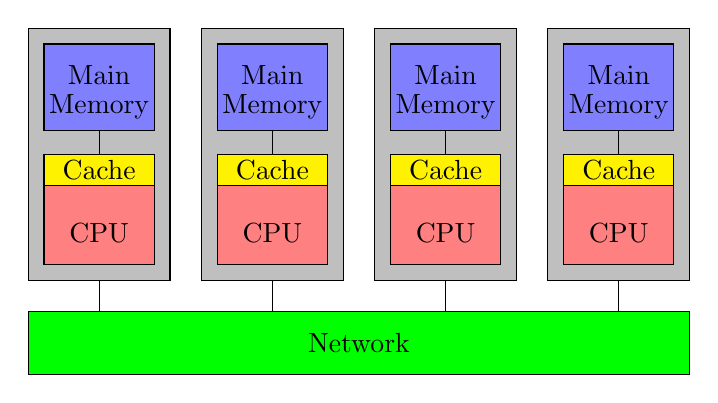
\begin{tikzpicture}[scale=0.4]
        \filldraw[fill=green] (0,-1) rectangle (21,-3);
        \draw (10.5,-2.0) node {Network};
        % First Node
        \filldraw[fill=gray!50!white] (0,0) rectangle (4.5,8);
        \filldraw[fill=blue!50!white] (0.5,4.75) rectangle (4.0,7.5);
        \filldraw[fill=yellow] (0.5,3.0) rectangle (4.0,4,0);
        \filldraw[fill=red!50!white] (0.5,0.5) rectangle (4.0,3.0);
        \draw (2.25,4.0) -- (2.25,4.75);
        \draw (2.25,0) -- (2.25,-1);
        \draw (2.25,6.5) node {Main};
        \draw (2.25,5.5) node {Memory};
        \draw (2.25,1.5) node {CPU};
        \draw (2.25,3.5) node {Cache};
        
        % Second Node
        \filldraw[fill=gray!50!white] (5.5,0) rectangle (10.0,8);
        \filldraw[fill=blue!50!white] (6.0,4.75) rectangle (9.5,7.5);
        \filldraw[fill=yellow] (6.0,3.0) rectangle (9.5,4,0);
        \filldraw[fill=red!50!white] (6.0,0.5) rectangle (9.5,3.0);
        \draw (7.75,4.0) -- (7.75,4.75);
        \draw (7.75,0) -- (7.75,-1);
        \draw (7.75,6.5) node {Main};
        \draw (7.75,5.5) node {Memory};
        \draw (7.75,1.5) node {CPU};
        \draw (7.75,3.5) node {Cache};
        
        % Third Node
        \filldraw[fill=gray!50!white] (11.0,0) rectangle (15.5,8);
        \filldraw[fill=blue!50!white] (11.5,4.75) rectangle (15.0,7.5);
        \filldraw[fill=yellow] (11.5,3.0) rectangle (15.0,4,0);
        \filldraw[fill=red!50!white] (11.5,0.5) rectangle (15.0,3.0);
        \draw (13.25,4.0) -- (13.25,4.75);
        \draw (13.25,0) -- (13.25,-1);
        \draw (13.25,6.5) node {Main};
        \draw (13.25,5.5) node {Memory};
        \draw (13.25,1.5) node {CPU};
        \draw (13.25,3.5) node {Cache};
        
        % Fourth Node
        \filldraw[fill=gray!50!white] (16.5,0) rectangle (21.0,8);
        \filldraw[fill=blue!50!white] (17.0,4.75) rectangle (20.5,7.5);
        \filldraw[fill=yellow] (17.0,3.0) rectangle (20.5,4,0);
        \filldraw[fill=red!50!white] (17.0,0.5) rectangle (20.5,3.0);
        \draw (18.75,4.0) -- (18.75,4.75);
        \draw (18.75,0) -- (18.75,-1);
        \draw (18.75,6.5) node {Main};
        \draw (18.75,5.5) node {Memory};
        \draw (18.75,1.5) node {CPU};
        \draw (18.75,3.5) node {Cache};
      \end{tikzpicture}
    \end{center}
\end{frame}

\begin{frame}
  \frametitle{Shared Memory Model}
%  \begin{columns}
%    \column{6cm}
    \begin{itemize}
      \item All threads can access the global memory space.
      \item Data sharing achieved via writing to/reading from the same memory location
      \item Example
      \begin{itemize}
        \item OpenMP
        \item Pthreads
      \end{itemize}
    \end{itemize}
%    \column{6cm}
    \begin{center}
      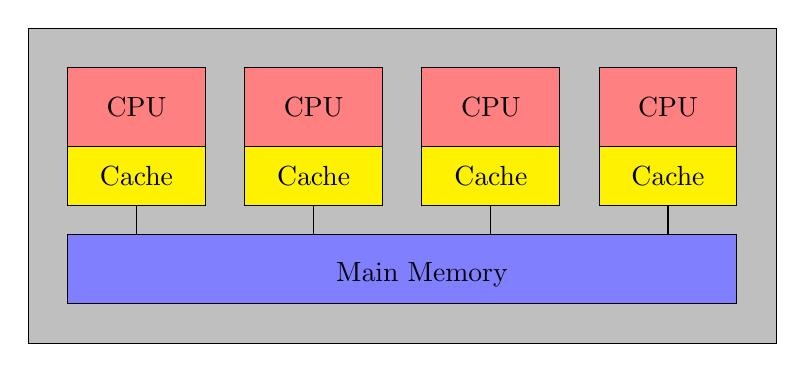
\begin{tikzpicture}[scale=0.5]
        \filldraw[fill=gray!50!white] (0,0) rectangle (19,8);
        \filldraw[fill=blue!50!white] (1,1) rectangle (18,2.75);
        \draw (10,1.75) node {Main Memory};
        % First Core
        \filldraw[fill=yellow] (1,3.5) rectangle (4.5,5.0);
        \draw (2.75,4.25) node {Cache};
        \filldraw[fill=red!50!white] (1,5.0) rectangle (4.5,7.0);
        \draw (2.75,6.0) node {CPU};
        \draw (2.75,3.5) -- (2.75,2.75);
        % Second Core
        \filldraw[fill=yellow] (5.5,3.5) rectangle (9.0,5.0);
        \draw (7.25,4.25) node {Cache};
        \filldraw[fill=red!50!white] (5.5,5.0) rectangle (9.0,7.0);
        \draw (7.25,6.0) node {CPU};
        \draw (7.25,3.5) -- (7.25,2.75);
        % Third Core
        \filldraw[fill=yellow] (10.0,3.5) rectangle (13.5,5.0);
        \draw (11.75,4.25) node {Cache};
        \filldraw[fill=red!50!white] (10.0,5.0) rectangle (13.5,7.0);
        \draw (11.75,6.0) node {CPU};
        \draw (11.75,3.5) -- (11.75,2.75);
        % Fourth Core
        \filldraw[fill=yellow] (14.5,3.5) rectangle (18.0,5.0);
        \draw (16.25,4.25) node {Cache};
        \filldraw[fill=red!50!white] (14.5,5.0) rectangle (18.0,7.0);
        \draw (16.25,6.0) node {CPU};
        \draw (16.25,3.5) -- (16.25,2.75);
      \end{tikzpicture}
%      \includegraphics[width=8cm]{./shared}
    \end{center}
%  \end{columns}
\end{frame}


\begin{frame}
  \frametitle{Clusters of SMP nodes}
  \begin{itemize}
    \item The shared memory model is most commonly represented by Symmetric Multi-Processing (SMP) systems
    \begin{itemize}
      \item Identical processors
      \item Equal access time to memory
    \end{itemize}
    \item Large shared memory systems are rare, clusters of SMP nodes are popular.
  \end{itemize}
%  \begin{columns}
%    \column{13cm}
%    \begin{center}
%      \includegraphics[width=12cm]{./smp-cluster}
%    \end{center}
%  \end{columns}
%\end{frame}

%\begin{frame}
  \begin{center}
    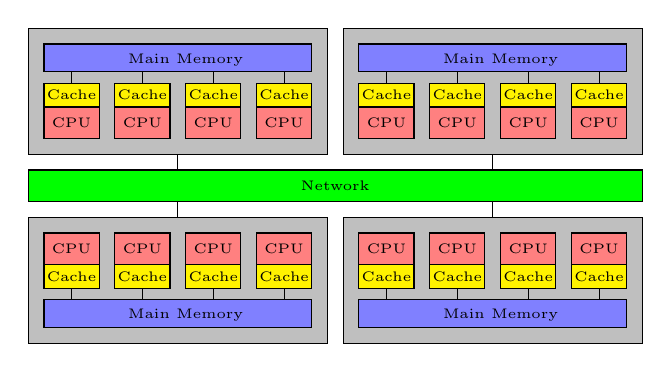
\begin{tikzpicture}[scale=0.2]
      \tikzstyle{every node}=[font=\tiny]
      \filldraw[fill=green] (0,9) rectangle (39,11);
      \draw (19.5,10) node {Network};
      % First Node
      \filldraw[fill=gray!50!white] (0,0) rectangle (19,8);
      \filldraw[fill=blue!50!white] (1,1) rectangle (18,2.75);
      \draw (10,1.75) node {Main Memory};
      % First Core
      \filldraw[fill=yellow] (1,3.5) rectangle (4.5,5.0);
      \draw (2.75,4.25) node {Cache};
      \filldraw[fill=red!50!white] (1,5.0) rectangle (4.5,7.0);
      \draw (2.75,6.0) node {CPU};
      \draw (2.75,3.5) -- (2.75,2.75);
      % Second Core
      \filldraw[fill=yellow] (5.5,3.5) rectangle (9.0,5.0);
      \draw (7.25,4.25) node {Cache};
      \filldraw[fill=red!50!white] (5.5,5.0) rectangle (9.0,7.0);
      \draw (7.25,6.0) node {CPU};
      \draw (7.25,3.5) -- (7.25,2.75);
      % Third Core
      \filldraw[fill=yellow] (10.0,3.5) rectangle (13.5,5.0);
      \draw (11.75,4.25) node {Cache};
      \filldraw[fill=red!50!white] (10.0,5.0) rectangle (13.5,7.0);
      \draw (11.75,6.0) node {CPU};
      \draw (11.75,3.5) -- (11.75,2.75);
      % Fourth Core
      \filldraw[fill=yellow] (14.5,3.5) rectangle (18.0,5.0);
      \draw (16.25,4.25) node {Cache};
      \filldraw[fill=red!50!white] (14.5,5.0) rectangle (18.0,7.0);
      \draw (16.25,6.0) node {CPU};
      \draw (16.25,3.5) -- (16.25,2.75);
      % Connect First Node to Network
      \draw (9.5,8) -- (9.5,9);

      % Second Node
      \filldraw[fill=gray!50!white] (20,0) rectangle (39,8);
      \filldraw[fill=blue!50!white] (21,1) rectangle (38,2.75);
      \draw (30,1.75) node {Main Memory};
      % First Core
      \filldraw[fill=yellow] (21,3.5) rectangle (24.5,5.0);
      \draw (22.75,4.25) node {Cache};
      \filldraw[fill=red!50!white] (21,5.0) rectangle (24.5,7.0);
      \draw (22.75,6.0) node {CPU};
      \draw (22.75,3.5) -- (22.75,2.75);
      % Second Core
      \filldraw[fill=yellow] (25.5,3.5) rectangle (29.0,5.0);
      \draw (27.25,4.25) node {Cache};
      \filldraw[fill=red!50!white] (25.5,5.0) rectangle (29.0,7.0);
      \draw (27.25,6.0) node {CPU};
      \draw (27.25,3.5) -- (27.25,2.75);
      % Third Core
      \filldraw[fill=yellow] (30.0,3.5) rectangle (33.5,5.0);
      \draw (31.75,4.25) node {Cache};
      \filldraw[fill=red!50!white] (30.0,5.0) rectangle (33.5,7.0);
      \draw (31.75,6.0) node {CPU};
      \draw (31.75,3.5) -- (31.75,2.75);
      % Fourth Core
      \filldraw[fill=yellow] (34.5,3.5) rectangle (38.0,5.0);
      \draw (36.25,4.25) node {Cache};
      \filldraw[fill=red!50!white] (34.5,5.0) rectangle (38.0,7.0);
      \draw (36.25,6.0) node {CPU};
      \draw (36.25,3.5) -- (36.25,2.75);
      % Connect Second Node to Network
      \draw (29.5,8) -- (29.5,9);

      % Third Node
      \filldraw[fill=gray!50!white] (0,12) rectangle (19,20);
      \filldraw[fill=blue!50!white] (1,17.25) rectangle (18,19);
      \draw (10,18.0) node {Main Memory};
      % First Core
      \filldraw[fill=yellow] (1,16.5) rectangle (4.5,15.0);
      \draw (2.75,15.75) node {Cache};
      \filldraw[fill=red!50!white] (1,15.0) rectangle (4.5,13.0);
      \draw (2.75,14.0) node {CPU};
      \draw (2.75,16.5) -- (2.75,17.25);
      % Second Core 
      \filldraw[fill=yellow] (5.5,16.5) rectangle (9.0,15.0);
      \draw (7.25,15.75) node {Cache};
      \filldraw[fill=red!50!white] (5.5,15.0) rectangle (9.0,13.0);
      \draw (7.25,14.0) node {CPU};
      \draw (7.25,16.5) -- (7.25,17.25);
      % Third Core 
      \filldraw[fill=yellow] (10.0,16.5) rectangle (13.5,15.0);
      \draw (11.75,15.75) node {Cache};
      \filldraw[fill=red!50!white] (10.0,15.0) rectangle (13.5,13.0);
      \draw (11.75,14.0) node {CPU};
      \draw (11.75,16.5) -- (11.75,17.25);
      % Fourth Core 
      \filldraw[fill=yellow] (14.5,16.5) rectangle (18.0,15.0);
      \draw (16.25,15.75) node {Cache};
      \filldraw[fill=red!50!white] (14.5,15.0) rectangle (18.0,13.0);
      \draw (16.25,14.0) node {CPU};
      \draw (16.25,16.5) -- (16.25,17.25);
      % Connect Third Node to Network
      \draw (9.5,11) -- (9.5,12);

      % Fourth Node
      \filldraw[fill=gray!50!white] (20,12) rectangle (39,20);
      \filldraw[fill=blue!50!white] (21,17.25) rectangle (38,19);
      \draw (30,18.0) node {Main Memory};
      % First Core
      \filldraw[fill=yellow] (21,16.5) rectangle (24.5,15.0);
      \draw (22.75,15.75) node {Cache};
      \filldraw[fill=red!50!white] (21,15.0) rectangle (24.5,13.0);
      \draw (22.75,14.0) node {CPU};
      \draw (22.75,16.5) -- (22.75,17.25);
      % Second Core 
      \filldraw[fill=yellow] (25.5,16.5) rectangle (29.0,15.0);
      \draw (27.25,15.75) node {Cache};
      \filldraw[fill=red!50!white] (25.5,15.0) rectangle (29.0,13.0);
      \draw (27.25,14.0) node {CPU};
      \draw (27.25,16.5) -- (27.25,17.25);
      % Third Core 
      \filldraw[fill=yellow] (30.0,16.5) rectangle (33.5,15.0);
      \draw (31.75,15.75) node {Cache};
      \filldraw[fill=red!50!white] (30.0,15.0) rectangle (33.5,13.0);
      \draw (31.75,14.0) node {CPU};
      \draw (31.75,16.5) -- (31.75,17.25);
      % Fourth Core 
      \filldraw[fill=yellow] (34.5,16.5) rectangle (38.0,15.0);
      \draw (36.25,15.75) node {Cache};
      \filldraw[fill=red!50!white] (34.5,15.0) rectangle (38.0,13.0);
      \draw (36.25,14.0) node {CPU};
      \draw (36.25,16.5) -- (36.25,17.25);
      % Connect Fourth Node to Network
      \draw (29.5,11) -- (29.5,12);
      
    \end{tikzpicture}
  \end{center}
\end{frame}

\begin{frame}
  \frametitle{Shared vs Distributed}
%  \begin{columns}
%    \column{5cm}
    \vspace{-0.5cm}
    \begin{exampleblock}{Shared Memory}
      \begin{itemize}
        \item Pros
        \begin{itemize}
          \item Global address space is user friendly
          \item Data sharing is fast
        \end{itemize}
        \item Cons
        \begin{itemize}
          \item Lack of scalability
          \item Data conflict issues
        \end{itemize}
      \end{itemize}
    \end{exampleblock}
%    \column{5cm}
    \begin{exampleblock}{Distributed Memory}
      \begin{itemize}
        \item Pros
        \begin{itemize}
          \item Memory scalable with number of processors
          \item Easier and cheaper to build
        \end{itemize}
        \item Cons
        \begin{itemize}
          \item Difficult load balancing
          \item Data sharing is slow
        \end{itemize}
      \end{itemize}
    \end{exampleblock}
%  \end{columns}
\end{frame}

\begin{frame}
  \frametitle{Why MPI?}
  \begin{itemize}
    \item \bflub{Standardization}: MPI is the only message passing library that can be considered a standard. It is supported on virtually all HPC platforms.
    \item \bflub{Portability}: There is little or no need to modify your source code when you port your application to a different platform.
    \item \bflub{Performance Opportunities}: Vendor implementations should be able to exploit native hardware features to optimize performance. Any implementation is free to develop optimized algorithms.
    \item \bflub{Functionality}: There are over 430 routines defined in MPI-3, which includes the majority of those in MPI-2 and MPI-1.
    \item[] Most MPI programs can be written using a dozen or less routines
    \item \bflub{Availability}: A variety of implementations are available, both vendor and public domain.
  \end{itemize}
%    \item There are already network communication libraries
%    \item Optimized for performance
%    \item Take advantage of faster network transport
%      \begin{itemize}
%        \item Shared memory (within a node)
%        \item Faster cluster interconnects (e.g. InfiniBand)
%        \item TCP/IP if all else fails
%      \end{itemize}
%    \item Enforces certain guarantees
%      \begin{itemize}
%      \item Reliable messages
%      \item In-order message arrival
%      \end{itemize}
%    \item Designed for multi-node technical computing
%  \end{itemize}
\end{frame}

\begin{frame}
  \frametitle{What is MPI?}
  \begin{itemize}
    \item MPI defines a standard API for message passing
      \begin{itemize}
        \item The standard includes
          \begin{itemize}
          \item What functions are available
          \item The syntax of those functions
          \item What the expected outcome is when calling those functions
          \end{itemize}
        \item The standard does NOT include
          \begin{itemize}
            \item Implementation details (e.g. how the data transfer occurs)
            \item Runtime details (e.g. how many processes the code run with  etc.)
          \end{itemize}
      \end{itemize}
    \item MPI provides C/C++ and Fortran bindings
  \end{itemize}
\end{frame}

\begin{frame}
  \frametitle{MPI Implementations}
  \begin{itemize}
    \item There are two different types of MPI implementations commonly used. 
    \begin{enumerate}
       \item \bflub{MPICH}: Developed by Argonne National Laboratory. 
       \begin{itemize}
           \item default MPI on Hawk.
           \item used as a starting point for various commercial and open source MPI libraries
           \item \bflub{MVAPICH2}: Developed by D. K. Panda with support for  InfiniBand, iWARP, RoCE, and Intel Omni-Path. 
           \item[] default MPI on Sol.
           \item \bflub{Intel MPI}: Intel's version of MPI. 
           \item[] available as part of the Intel OneAPI HPC Toolkit
           \item \bflub{IBM MPI}:  for IBM BlueGene, and 
           \item \bflub{CRAY MPI}: for Cray systems.
       \end{itemize}
       \item \bflub{OpenMPI}: A Free, Open Source implementation from merger of three well know MPI implementations. 
       \begin{itemize}
           \item \bflub{FT-MPI} from the University of Tennessee,
           \item \bflub{LA-MPI}: from Los Alamos National Laboratory,
           \item \bflub{LAM/MPI}: from Indiana University
           \item Can be used for commodity network as well as high speed network.
           \item available on Sol and Hawk but only libraries and a couple of packages are available.
       \end{itemize}
    \end{enumerate}
  \end{itemize}
\end{frame}

\begin{frame}[fragile]
  \frametitle{MPI Compilers}
  \begin{itemize}
    \item There is no MPI compiler available to compile programs nor is there is a compiler flag.
    \item Instead, you need to build the MPI libraries for a particular compiler.
    \item You can use MVAPICH2 and MPICH on Sol
    \item You should only use MPICH on Hawk. 
    \item Each of these builds provide \lstC{mpicc}, \lstC{mpicxx} and \lstC{mpif90} for compiling C, C++ and Fortran codes respectively that are wrapper for the underlying compilers
  \end{itemize}
  \vspace{-0.25cm}
  \begin{block}{}
    \begin{lstlisting}[basicstyle=\tiny\ttfamily]
[alp514.sol](793): module load mvapich2
[alp514.sol](794): mpicc -show
/share/Apps/intel/2020/compilers_and_libraries_2020.3.275/linux/bin/intel64/icc -lmpi -I/share/Apps/lusoft/opt/spack/linux-centos8-haswell/intel-20.0.3/mvapich2/2.3.4-wguydha/include -L/share/Apps/lusoft/opt/spack/linux-centos8-haswell/intel-20.0.3/mvapich2/2.3.4-wguydha/lib -Wl,-rpath -Wl,/share/Apps/lusoft/opt/spack/linux-centos8-haswell/intel-20.0.3/mvapich2/2.3.4-wguydha/lib
[alp514.sol](795): module load mpich

Lmod is automatically replacing "mvapich2/2.3.4" with "mpich/3.3.2".

[alp514.sol](796): mpif90 -show
/share/Apps/intel/2020/compilers_and_libraries_2020.3.275/linux/bin/intel64/ifort -L/share/Apps/lusoft/opt/spack/linux-centos8-haswell/intel-20.0.3/hwloc/2.2.0-rjrzfy7/lib -I/share/Apps/lusoft/opt/spack/linux-centos8-haswell/intel-20.0.3/mpich/3.3.2-n7f36fo/include -I/share/Apps/lusoft/opt/spack/linux-centos8-haswell/intel-20.0.3/mpich/3.3.2-n7f36fo/include -L/share/Apps/lusoft/opt/spack/linux-centos8-haswell/intel-20.0.3/mpich/3.3.2-n7f36fo/lib -lmpifort -Wl,-rpath -Wl,/share/Apps/lusoft/opt/spack/linux-centos8-haswell/intel-20.0.3/mpich/3.3.2-n7f36fo/lib -lmpi
    \end{lstlisting}
  \end{block}
\end{frame}

\begin{frame}[fragile,allowframebreaks]
  \frametitle{Running MPI Applications}
  \begin{itemize}
  \item To run MPI applications, you need to launch the application using 
    \begin{itemize}
       \item \lstC{mpirun} (OpenMPI), 
       \item \lstC{mpirun\_rsh} (MPICH and MVAPICH2), or 
       \item \lstC{mpiexec} (OpenMPI, MPICH and MVAPICH2).
    \end{itemize}
  \item \lstC{mpirun}, \lstC{mpirun\_rsh} and \lstC{mpiexec} are schedulers for the MPI library.
  \item On clusters with SLURM scheduler, \lstC{srun} can be used to launch MPI applications
  \item The MPI scheduler needs to be given additional information to correctly run MPI applications
  \end{itemize}
  \begin{center}
   \small{
    \begin{tabular}{|faaa|}
      \hline
      \rowcolor{lublue}& mpiexec & mpirun\_rsh & mpirun \\
      \hline
      \# Processors & -n numprocs & -n numprocs & -np numprocs \\
      Processors List & -hosts core1,core2,... & core1 core2 ... & -hosts core1,core2,... \\
      Processor filelist & -f file & -hostfile file & -f/-hostfile file \\
      \hline
    \end{tabular}
  }
  \end{center}
  \framebreak
  \begin{itemize}
    \item Run an application myapp on 72 processors on a total of 3 nodes - node1, node2 and node3 
      \begin{itemize}
        \item \lstC{mpirun}: \texttt{mpirun -np 72  -f filename myapp}
        \item \lstC{mpirun\_rsh}: \texttt{mpirun\_rsh -np 72  -hostfile filename myapp}
        \item \lstC{mpiexec}: \texttt{mpiexec -n 72  -hosts node1,node2,node3  -ppn 24 myapp}
      \end{itemize}
    \item The SLURM scheduler's \lstC{srun} launcher has information needed to run a mpi job
      \begin{itemize}
        \item \lstC{srun}: \texttt{srun myapp}
      \end{itemize}
  \end{itemize}
\end{frame}

\begin{frame}[fragile, allowframebreaks]{MPI Program Structure}
  \begin{center}
    \vspace{-0.5cm}
    \includegraphics[height=0.8\textheight]{../slides/image/parprog/prog_structure}
  \end{center}
  \framebreak
  \begin{itemize}
    \item Header File: Required for all programs that make MPI library calls.
      \begin{center}
        \begin{tabular}{|a|a|}
          \hline
          \rowcolor{lublue}C & Fortran \\
          \hline
          \lstC{#include "mpi.h"} & \lstfortran{include 'mpif.h'} OR \lstfortran{use mpi} \\
          \hline
        \end{tabular}
      \end{center}
    \item Format of MPI Calls:
      \begin{itemize}
        \item C names are case sensitive; Fortran names are not.
        \item Programs must not declare variables or functions 
          with names beginning with the prefix MPI\_ or PMPI\_ (profiling interface)
      \end{itemize}
      \begin{center}
        \begin{tabular}{|f|a|}
          \hline
          \rowcolor{lublue}\multicolumn{2}{|c|}{C Binding}\\
          \hline
          Format & \lstC{rc = MPI_Xxxxx(parameter, ... )} \\
          Example & \lstC{rc = MPI_Bsend(\&buf,count,type,dest,tag,comm)} \\
          Error code & Returned as "rc". MPI\_SUCCESS if successful \\
          \hline
          \rowcolor{lublue}\multicolumn{2}{|c|}{Fortran Binding}\\
          \hline
          Format & \lstfortran{call mpi_xxxxx(parameter,..., ierr)}\\
          Example & \lstfortran{CALL MPI_BSEND(buf,count,type,dest,tag,comm,ierr)} \\
          Error code & Returned as  "ierr" parameter. MPI\_SUCCESS if successful \\
          \hline
        \end{tabular}
      \end{center}
  \framebreak
  \item MPI uses objects called communicators and groups to define which collection of processes may communicate with each other.
  \item Most MPI routines require you to specify a communicator as an argument.
  \item \lstC{MPI_COMM_WORLD}: the default communicator contains all processes running a MPI program.
    \begin{center}
      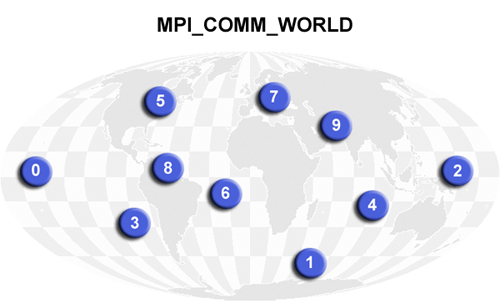
\includegraphics[width=0.5\textwidth]{../slides/image/parprog/comm_world}      
    \end{center}
  \item Every process has its own unique, integer identifier assigned, called rank, by the system when the process initializes
  \end{itemize}
\end{frame}

\begin{frame}[fragile, allowframebreaks]
  \frametitle{Environment management functions}
  \begin{itemize}
    \item \bflub{{MPI\_INIT}}: Initialize the MPI environment
    \item \bflub{{MPI\_COMM\_SIZE}}: Return total number of MPI processes
    \item \bflub{{MPI\_COMM\_RANK}}: Return rank of calling process
    \item \bflub{{MPI\_ABORT}}: Terminates all MPI processes
    \item \bflub{{MPI\_GET\_PROCESSOR\_NAME}}: Returns the processor name.
    \item \bflub{{MPI\_GET\_VERSION}}: Returns the version and subversion of the MPI standard
    \item \bflub{{MPI\_INITIALIZED}}: Indicates whether MPI\_Init has been called
    \item \bflub{{MPI\_WTIME}}: Returns an elapsed wall clock time in seconds
    \item \bflub{{MPI\_WTICK}}: Returns the resolution in seconds of MPI\_WTIME
    \item \bflub{{MPI\_FINALIZE}}: Terminate the MPI environment
  \end{itemize}
  \framebreak
  \vspace{-0.5cm}
  \begin{columns}
    \column{0.45\textwidth}
    \begin{exampleblock}{C/C++}
      \begin{lstlisting}[basicstyle=\scriptsize\ttfamily,language=C]
MPI_Init (&argc,&argv) 
MPI_Comm_size (comm,&size) 
MPI_Comm_rank (comm,&rank) 
MPI_Abort (comm,errorcode)
MPI_Get_processor_name (&name,&resultlength)
MPI_Get_version (&version,&subversion)
MPI_Initialized (&flag) 
MPI_Wtime ()
MPI_Wtick ()
MPI_Finalize ()
      \end{lstlisting}
    \end{exampleblock}
    \column{0.45\textwidth}
    \begin{exampleblock}{Fortran}
      \begin{lstlisting}[basicstyle=\scriptsize\ttfamily,language={[90]Fortran}]
MPI_INIT (ierr)
MPI_COMM_SIZE (comm,size,ierr)
MPI_COMM_RANK (comm,rank,ierr)
MPI_ABORT (comm,errorcode,ierr)
MPI_GET_PROCESSOR_NAME (name,resultlength,ierr)
MPI_GET_VERSION (version,subversion,ierr)
MPI_INITIALIZED (flag,ierr)
MPI_WTIME ()
MPI_WTICK ()
MPI_FINALIZE (ierr)
      \end{lstlisting}
    \end{exampleblock}
  \end{columns}
\end{frame}

%\begin{frame}
%  \frametitle{MPI Program Outline}
%  \begin{enumerate}
%    \item Initiate communication between processes
%      \begin{itemize}
%        \item \bflub{MPI\_INIT}: initialize MPI environment
%        \item \bflub{MPI\_COMM\_SIZE}: return total number of MPI processes
%        \item \bflub{MPI\_COMM\_RANK}: return rank of calling process
%      \end{itemize}
%      \item Communicate data between processes
%        \begin{itemize}
%          \item \bflub{MPI\_SEND}: send a message
%          \item \bflub{MPI\_RECV}: receive a message 
%        \end{itemize}
%      \item Terminate the MPI environment using \textbf{\textcolor{lubrown}{MPI\_FINALIZE}}
%  \end{enumerate}
%\end{frame}


\begin{frame}[fragile]{Example: Hellow World}
  \begin{columns}
    \column{0.45\textwidth}
    \vspace{-0.5cm}
    \begin{exampleblock}{C}
      \lstinputlisting[language=OmpC]{../slides/code/parprog/src/mpi/helloworld.c}
    \end{exampleblock}
    \column{0.45\textwidth}
    \vspace{-0.5cm}
    \begin{exampleblock}{Fortran}
      \lstinputlisting[language={OmpFortran}]{../slides/code/parprog/src/mpi/helloworld.f90}
    \end{exampleblock}
  \end{columns}
\end{frame}

\begin{frame}{Exercise: Writing your first MPI program}
  \begin{itemize}
    \item Take the hello world code and add a few Environment Management functions
    \item Compile your code
    \item Run your code several different ways
    \item[]
    \item Examples to try out
      \begin{enumerate}
        \item Print hostname
        \item Print mpi version
        \item Print hostname if your rank is odd and mpi version if rank is even 
      \end{enumerate}
  \end{itemize}
\end{frame}

\begin{frame}{First MPI Program}
  \begin{columns}
    \column{0.45\textwidth}
    \vspace{-0.5cm}
    \begin{exampleblock}{C}
      \lstinputlisting[language=OmpC]{../slides/code/parprog/src/mpi/hello.c}
    \end{exampleblock}
    \column{0.45\textwidth}
    \vspace{-0.5cm}
    \begin{exampleblock}{Fortran}
      \lstinputlisting[language={OmpFortran}]{../slides/code/parprog/src/mpi/hello.f90}
    \end{exampleblock}
  \end{columns}
\end{frame}

\begin{frame}[fragile]
  \frametitle{Compile \& Run}
  \begin{exampleblock}{}
    \begin{lstlisting}[basicstyle=\scriptsize\ttfamily]
[alp514.sol](1024): module load intel mpich

Lmod is automatically replacing ``mvapich2/2.3.4'' with ``mpich/3.3.2''.

[alp514.sol](1025): mpicc -o helloc hello.c
[alp514.sol](1026): mpif90 -o hellof hello.f90
[alp514.sol](1027): srun -p hawkgpu -n 4 -t 10 ./hellof
Number of tasks= 4 My rank= 0 Running on hawk-b624.cc.lehigh.edu
Number of tasks= 4 My rank= 1 Running on hawk-b624.cc.lehigh.edu
Number of tasks= 4 My rank= 3 Running on hawk-b624.cc.lehigh.edu
Number of tasks= 4 My rank= 2 Running on hawk-b624.cc.lehigh.edu

[alp514.sol](1028): srun -p hawkgpu -n 4 -t 10 ./helloc
Number of tasks= 4 My rank= 0 Running on hawk-b624.cc.lehigh.edu
Number of tasks= 4 My rank= 1 Running on hawk-b624.cc.lehigh.edu
Number of tasks= 4 My rank= 3 Running on hawk-b624.cc.lehigh.edu
Number of tasks= 4 My rank= 2 Running on hawk-b624.cc.lehigh.edu

[alp514.sol](1031): srun -p lts -n 4 -N 4 -t 10 ./helloc
Number of tasks= 4 My rank= 0 Running on sol-a105.cc.lehigh.edu
Number of tasks= 4 My rank= 2 Running on sol-a107.cc.lehigh.edu
Number of tasks= 4 My rank= 3 Running on sol-a108.cc.lehigh.edu
Number of tasks= 4 My rank= 1 Running on sol-a106.cc.lehigh.edu
    \end{lstlisting}
  \end{exampleblock}
\end{frame}

\begin{frame}
  \frametitle{Compiling MPI Programs}
  \begin{itemize}
    \item Not a part of the standard
      \begin{itemize}
        \item Could vary from platform to platform
        \item Or even from implementation to implementation on the same  platform
        \item mpicc/mpicxx/mpif77/mpif90: wrappers to compile MPI code and auto 
          link to startup and message passing libraries 
      \end{itemize}
    \item<2> \alert<2>{Unlike OpenMP and OpenACC, you cannot compile a MPI program 
      for running in serial using the serial compiler}
    \item<2> \alert<2>{The MPI program is not a standard C/C++/Fortran program and 
      will spit out errors about missing libraries} 
  \end{itemize}
\end{frame}

%\begin{frame}[fragile]
%  \frametitle{Communicators}
%  \begin{itemize}
%  \item A communicator is an identifier associated with a  group of processes
%    \only<1>{
%      \begin{center}
%        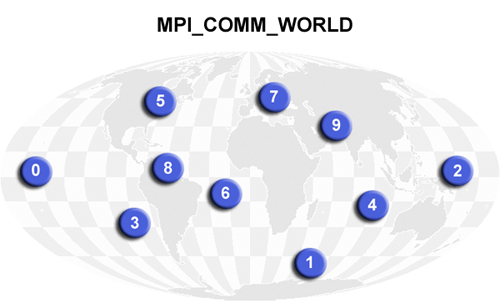
\includegraphics[width=0.5\textwidth]{../slides/image/parprog/comm_world}      
%      \end{center}
%      \lstC{MPI_Comm_size(MPI_COMM_WORLD,int \&numtasks);}\\
%      \lstC{MPI_Comm_rank(MPI_COMM_WORLD,int \&rank);}\\
%      \vspace{0.5cm}
%      \lstfortran{call MPI_COMM_SIZE(MPI_COMM_WORLD, numtasks, ierr)}\\
%      \lstfortran{call MPI_COMM_RANK(MPI_COMM_WORLD, rank, ierr)}
%    }
%    \only<2->{
%      \begin{itemize}
%      \item Can be regarded as the name given to an ordered list of processes
%      \item Each process has a unique rank, which starts from 0 
%        (usually referred to as "root")
%      \item It is the context of MPI communications and operations
%        \begin{itemize}
%        \item For instance, when a function is called to send data to all 
%          processes, MPI needs to understand what "all" 
%        \end{itemize}
%      \item \lstC{MPI_COMM_WORLD}: the default communicator contains all processes 
%        running a MPI program
%      \item There can be many communicators
%        \begin{itemize}
%        \item e.g., \lstC{MPI_Comm_split(MPI_Commcomm, intcolor, int, kye, 
%          MPI_Comm* newcomm)}
%        \end{itemize}
%      \item A process can belong to multiple communicators
%        \begin{itemize}
%        \item The rank is usually different
%        \end{itemize}
%      \end{itemize}
%    }
%  \end{itemize}
%\end{frame}

\begin{frame}[fragile]
  \frametitle{Communicator Information}
  \begin{itemize}
  \item \lstC{MPI_COMM_WORLD}: the default communicator contains all processes running a MPI program.
    \begin{center}
      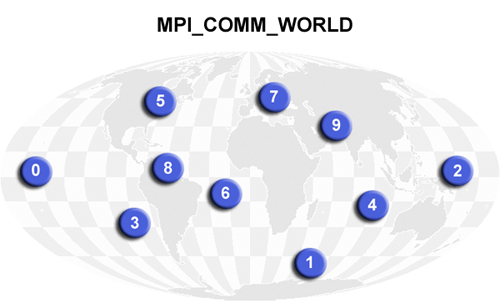
\includegraphics[width=0.5\textwidth]{../slides/image/parprog/comm_world}      
    \end{center}
  \item Rank: unique id of each process
    \begin{itemize}
    \item \textcolor{lubrown}{C:} \lstC{MPI_Comm_Rank(MPI_Comm comm, int *rank)}
    \item \textcolor{lubrown}{Fortran:} \lstfortran{MPI_COMM_RANK(COMM, RANK, ERR)}
    \end{itemize}
  \item Get the size/processes of a communicator
    \begin{itemize}
    \item \textcolor{lubrown}{C:} \lstC{MPI_Comm_Size(MPI_Comm comm, int *size)}
    \item \textcolor{lubrown}{Fortran:} \lstfortran{MPI_COMM_SIZE(COMM, SIZE, ERR)}
    \end{itemize}
  \end{itemize}
\end{frame}

\begin{frame}[fragile, allowframebreaks]
  \frametitle{Communicator Functions}
  \begin{itemize}
  \item Point-to-point communication functions
    \begin{itemize}
    \item Message transfer from one process to another
    \end{itemize}
  \item Collective communication functions 
    \begin{itemize}
    \item Message transfer involving all processes in a communicator
    \end{itemize}
  \end{itemize}
  \begin{columns}
    \column{0.4\textwidth}
    \begin{center}
      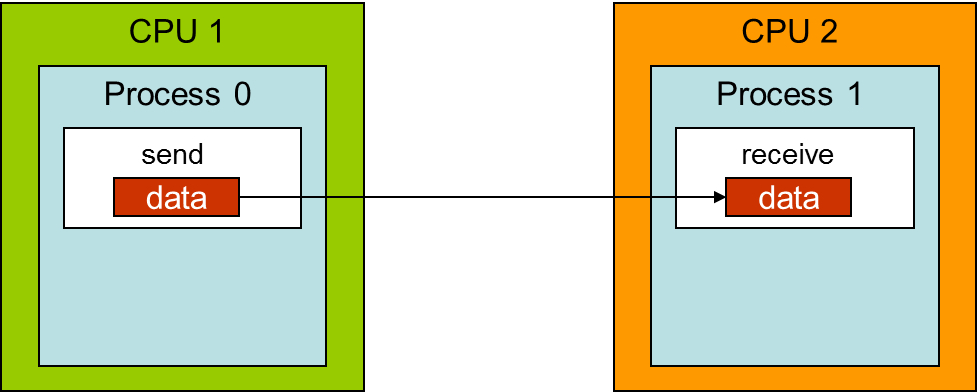
\includegraphics[width=\textwidth]{../slides/image/parprog/SimpleSendAndRecv}
    \end{center}
    \column{0.4\textwidth}
    \begin{center}
      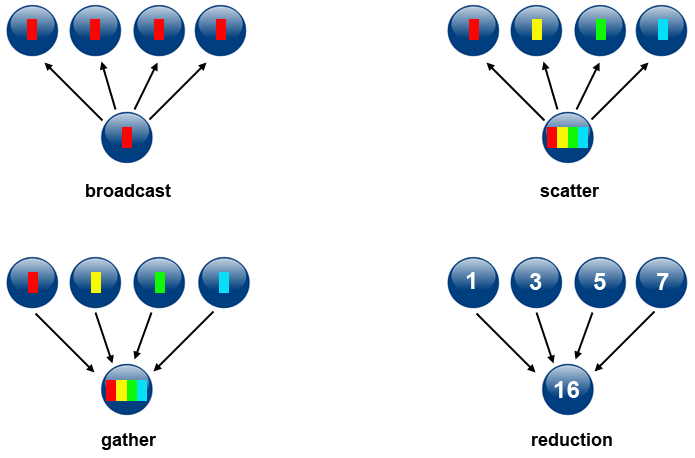
\includegraphics[width=\textwidth]{../slides/image/parprog/collective_comm}
    \end{center}
  \end{columns}
\end{frame}

\begin{frame}[fragile]
  \frametitle{Point-to-point Communication}
  \begin{itemize}
  \item MPI point-to-point operations typically involve message passing between two, and only two, different MPI tasks. 
  \item One task is performing a send operation and the other task is performing a matching receive operation.
  \item There are different types of send and receive routines used for different purposes.
    \begin{enumerate}
    \item Blocking send / blocking receive
    \item Non-blocking send / non-blocking receive
    \item Synchronous send
    \end{enumerate}
  \end{itemize}
\end{frame}

\begin{frame}[allowframebreaks]{Buffering}
  \begin{itemize}
    \item Ideally, every send operation would be perfectly synchronized with its matching receive.
    \item MPI implementation must be able to deal with storing data when the two tasks are out of sync.
    \item Consider the following two cases:
      \begin{enumerate}
        \item A send operation occurs 5 seconds before the receive is ready - where is the message while the receive is pending?
        \item Multiple sends arrive at the same receiving task which can only accept one send at a time - what happens to the messages that are “backing up”?
      \end{enumerate}
    \item MPI implementation (not the MPI standard) decides what happens to data in these types of cases. 
    \item Typically, a system buffer area is reserved to hold data in transit.
  \end{itemize}
  \centering{
    \includegraphics[width=0.4\textwidth]{../slides/image/parprog/buffer_recv}
    }
  \begin{block}{System buffer space}
    \begin{itemize}
      \item Opaque to the programmer and managed entirely by the MPI library
      \item A finite resource that can be easy to exhaust
      \item Often mysterious and not well documented
      \item Able to exist on the sending side, the receiving side, or both
      \item Something that may improve program performance because it allows send - receive operations to be asynchronous.
    \end{itemize}
  \end{block}
\end{frame}

\begin{frame}[allowframebreaks]{Blocking vs. Non-blocking}
  \begin{block}{Blocking send / receive }
    \begin{itemize}
      \item send will "return" after it is safe to modify the application buffer (your send data) for reuse
      \item send can be synchronous i.e. handshake with the receive task to confirm a safe send.
      \item send can be asynchronous if a system buffer is used to hold the data for eventual delivery to the receive.
      \item receive only "returns" after the data has arrived and is ready for use by the program.
    \end{itemize}
  \end{block}

  \framebreak

  \begin{block}{Non-blocking send / receive}
    \begin{itemize}
      \item behave similarly - they will return almost immediately. 
      \item do not wait for any communication events to complete, such as message copying from user memory to system buffer space or the actual arrival of message.
      \item operations simply "request" the MPI library to perform the operation when it is able. 
      \item[] The user can not predict when that will happen.
      \item communications are primarily used to overlap computation with communication and exploit possible performance gains.
    \end{itemize}
  \end{block}

  \framebreak

  \begin{block}{Order}
    \begin{itemize}
      \item MPI guarantees that messages will not overtake each other.
      \item If a sender sends two messages (Message 1 and Message 2) in succession to the same destination, and both match the same receive, the receive operation will receive Message 1 before Message 2.
      \item If a receiver posts two receives (Receive 1 and Receive 2), in succession, and both are looking for the same message, Receive 1 will receive the message before Receive 2.
      \item Order rules do not apply if there are multiple threads participating in the communication operations.
    \end{itemize}
  \end{block}
  \begin{block}{Fairness}
    \begin{itemize}
      \item MPI does not guarantee fairness - it’s up to the programmer to prevent “operation starvation”.
    \end{itemize}
    \centering{
      \includegraphics[width=0.5\textwidth]{../slides/image/parprog/fairness}
    }
  \end{block}
\end{frame}

\begin{frame}[fragile,allowframebreaks]{Point-to-point Communication Functions}
  \begin{block}{Blocking send / receive}
    \begin{itemize}
      \item \textbf{MPI\_Send}: Basic blocking send operation
      \item Routine returns only after the application buffer in the sending task is free for reuse.
      \item[] \lstC{MPI_Send (\&buf,count,datatype,dest,tag,comm) }
      \item[] \lstfortran{MPI_SEND (buf,count,datatype,dest,tag,comm,ierr)}
    \end{itemize}

    \begin{itemize}
      \item \textbf{MPI\_Recv}: Receive a message 
      \item will block until the requested data is available in the application buffer in the receiving task.
      \item[] \lstC{MPI_Recv (\&buf,count,datatype,source,tag,comm,\&status) }
      \item[] \lstfortran{MPI_RECV (buf,count,datatype,source,tag,comm,status,ierr)}
    \end{itemize}
  \end{block}

  \framebreak

  \begin{block}{Non-blocking send / receive}
    \begin{itemize}
      \item \textbf{MPI\_Isend}: Identifies an area in memory to serve as a send buffer.
      \item Processing continues immediately without waiting for the message to be copied out from the application buffer
      \item[] \lstC{MPI_Isend (\&buf,count,datatype,dest,tag,comm,\&request) }
      \item[] \lstfortran{MPI_ISEND (buf,count,datatype,dest,tag,comm,request,ierr)}
      \item \textbf{MPI\_Irecv}: Identifies an area in memory to serve as a receive buffer
      \item Processing continues immediately without actually waiting for the message to be received and copied into the the application buffer
      \item[] \lstC{MPI_Irecv (\&buf,count,datatype,source,tag,comm,\&request)}
      \item[] \lstfortran{MPI_IRECV (buf,count,datatype,source,tag,comm,request,ierr)}
      \item \textbf{MPI\_WAIT} and \textbf{MPI\_TEST}: Functions required by nonblocking send and receive use to determine when the non-blocking receive operation completes and the requested message is available in the application buffer.
    \end{itemize}
  \end{block}
\end{frame}

\begin{frame}[fragile,allowframebreaks]{Point-to-Point Communication Function Arguments}
  \begin{itemize}
    \item \lstC{buf}: address space that references the data that is to be sent or received
    \item[] In most cases, variable name that is to be sent/received
    \item[] C programs: this argument is passed by reference and usually must be prepended with an ampersand: \&var1
    \item \lstC{count}: number of data elements of a particular type to be sent
    \item \lstC{datatype}: MPI predefines its elementary data types
      \begin{columns}
        \column{0.45\textwidth}
        {\footnotesize
          \begin{center}
            \begin{tabular}{|f|f|}
              \hline
              \rowcolor{lublue}C type  &   MPI type \\
              \hline
              char &   MPI\_CHAR \\
              unsigned char &   MPI\_UNSIGNED\_CHAR \\
              short &   MPI\_SHORT \\
              unsigned short &   MPI\_UNSIGNED\_SHORT \\
              int &   MPI\_INT \\
              unsigned int &   MPI\_UNSIGNED \\
              long int  &  MPI\_LONG \\
              unsigned long int &   MPI\_UNSIGNED\_LONG \\
              long long int  &  MPI\_LONG\_LONG\_INT \\
              float  &  MPI\_FLOAT \\
              double &   MPI\_DOUBLE \\
              long double &   MPI\_LONG\_DOUBLE \\
              unsigned char &   MPI\_BYTE \\
              \hline
            \end{tabular}
          \end{center}
          }
        \column{0.45\textwidth}
        {\footnotesize
          \begin{center}
            \begin{tabular}{|f|f|}
              \hline
              \rowcolor{lublue}Fortran type  &   MPI type \\
              \hline
              character(1) & MPI\_CHARACTER \\
              integer & MPI\_INTEGER \\
              integer*2 & MPI\_INTEGER2 \\
              integer*4 & MPI\_INTEGER4 \\
              real & MPI\_REAL \\
              real*4 & MPI\_REAL4 \\
              real*8 & MPI\_REAL8 \\
              double precision & MPI\_DOUBLE\_PRECISION \\
              complex & MPI\_COMPLEX \\
              double complex & MPI\_DOUBLE\_COMPLEX \\
              \hline
            \end{tabular}
          \end{center}
        }
      \end{columns}
      \framebreak
    \item \lstC{dest}: indicates the process where a message should be delivered
    \item[] specified as the rank of the receiving process
    \item \lstC{source}: indicates the originating process of the message.
      \item[] specified as the rank of the sending process
    \item \lstC{tag}: arbitrary non-negative integer assigned by the programmer to uniquely identify a message
    \item[] send and receive operations should match message tags
    \item[] for a receive operation, the wild card \lstC{MPI\_ANY\_TAG} can be used to receive any message regardless of its tag.
    \item \lstC{comm}: indicates the communication context, or set of processes for which the source or destination fields are valid 
    \item[] unless the programmer is explicitly creating new communicators, the predefined communicator \lstC{MPI\_COMM\_WORLD} is usually used
      \framebreak
    \item \lstC{status}: for a receive operation, indicates the source of the message and the tag of the message.
    \item[] C: pointer to a predefined structure \lstC{MPI\_Status}
    \item[] Fortran: integer array of size \lstC{MPI\_STATUS\_SIZE}
    \item \lstC{request}: used by non-blocking send and receive operations
    \item[] since non-blocking operations may return before the requested system buffer space is obtained, the system issues a unique “request number”
    \item[] programmer uses this system assigned “handle” later determine completion of the non-blocking operation
    \item[] C: a pointer to a predefined structure \lstC{MPI\_Request}.
    \item[] Fortran: an integer
  \end{itemize}
\end{frame}

\begin{frame}[fragile,allowframebreaks]{Blocking Message Passing Funtions}
  \begin{itemize}
    \item \bflub{MPI\_Send}: Basic blocking send operation
    \item \bflub{MPI\_Recv}: Receive a message and block until the requested data is available in the application buffer in the receiving task.
    \item \bflub{MPI\_Ssend}: Synchronous blocking send: Send a message and block until the application buffer in the sending task is free for reuse and the destination process has started to receive the message
    \item \bflub{MPI\_Sendrecv}: Send a message and post a receive before blocking. 
    \item[] Will block until the sending application buffer is free for reuse and until the receiving application buffer contains the received message
    \framebreak
    \item \bflub{MPI\_Probe}: Performs a blocking test for a message. 
    \item[] The “wildcards” MPI\_ANY\_SOURCE and MPI\_ANY\_TAG may be used to test for a message from any source or with any tag. 
    \item[] \lstC{C}: the actual source and tag will be returned in the status structure as status.MPI\_SOURCE and status.MPI\_TAG. 
    \item[] \lstC{Fortran}: they will be returned in the integer array status(MPI\_SOURCE) and status(MPI\_TAG).
    \item \bflub{MPI\_Get\_Count}: Returns the source, tag and number of elements of datatype received. 
    \item[] Can be used with both blocking and non-blocking receive operations. 
    \item[] \lstC{C}: the actual source and tag will be returned in the status structure as status.MPI\_SOURCE and status.MPI\_TAG. 
    \item[] \lstC{Fortran}: they will be returned in the integer array status(MPI\_SOURCE) and status(MPI\_TAG).
  \end{itemize}
  \framebreak
  \vspace{-0.5cm}
  \begin{block}{}
  \begin{lstlisting}[basicstyle=\scriptsize\ttfamily,language=C]
MPI_Ssend (&buf,count,datatype,dest,tag,comm)
MPI_Sendrecv (&sendbuf,sendcount,sendtype,dest,sendtag,
  &recvbuf,recvcount,recvtype,source,recvtag,
  comm,&status)
MPI_Probe (source,tag,comm,&status)
MPI_Get_count (&status,datatype,&count)
  \end{lstlisting}
  \end{block}
  \vspace{-0.25cm}
  \begin{block}{}
  \begin{lstlisting}[basicstyle=\scriptsize\selectfont\ttfamily,language=Fortran]
MPI_SSEND (buf,count,datatype,dest,tag,comm,ierr)
MPI_SENDRECV (sendbuf,sendcount,sendtype,dest,sendtag,&
   recvbuf,recvcount,recvtype,source,recvtag,&
   comm,status,ierr)
MPI_PROBE (source,tag,comm,status,ierr)
MPI_GET_COUNT (status,datatype,count,ierr)
  \end{lstlisting}
  \end{block}
\end{frame}

\begin{frame}[fragile,allowframebreaks]{Exercise: Ping Pong}
  \begin{itemize}
    \item Modify the \lstC{pingpong.c} or \lstC{pingpong.f90} example to do a blocking send and recieve.
    \item Task 0 sends a ping to task 1 and awaits return ping
    \item This example only requires two MPI processes
    \item What happens if you run on more than 2 cpus
  \end{itemize}
  \framebreak
  \begin{exampleblock}{}
    \begin{lstlisting}[basicstyle=\scriptsize\ttfamily]
[alp514.sol](1132): mpicc -o pingpongc pingpong.c
[alp514.sol](1133): mpif90 -o pingpongf pingpong.f90
[alp514.sol](1134): srun -n 2 -p hawkgpu -t 5 ./pingpongc
Task 1: Received 1 char(s) from task 0 with tag 1
Task 0: Received 1 char(s) from task 1 with tag 1

[alp514.sol](1135): srun -n 2 -p hawkgpu -t 5 ./pingpongf
Task   1 : Received  1  char(s) from task  0 with tag  1
Task   0 : Received  1  char(s) from task  1 with tag  1

[alp514.sol](1136): srun -n 4 -p hawkgpu -t 5 ./pingpongf
Task   1 : Received  1  char(s) from task  0 with tag  1
Task   3 : Received  0  char(s) from task  0 with tag  0
Task   2 : Received  0  char(s) from task  0 with tag  0
Task   0 : Received  1  char(s) from task  1 with tag  1

[alp514.sol](1137): srun -n 4 -p hawkgpu -t 5 ./pingpongc
Task 0: Received 1 char(s) from task 1 with tag 1
Task 1: Received 1 char(s) from task 0 with tag 1
Task 2: Received -32766 char(s) from task 2496 with tag -1075053569
Task 3: Received -32766 char(s) from task 1668810496 with tag 32588
    \end{lstlisting}
  \end{exampleblock}
\end{frame}


\begin{frame}[fragile,allowframebreaks]{Non Blocking Message Passing Functions}
  \begin{itemize}
    \item \bflub{MPI\_ISend}: Identifies an area in memory to serve as a send buffer.
    \item[] Processing continues immediately without waiting for the message to be copied out from the application buffer. 
    \item[] A communication request handle is returned for handling the pending message status. 
    \item[] The program should not modify the application buffer until the non-blocking send has completed.
    \item \bflub{MPI\_Irecv}: Identifies an area in memory to serve as a receive buffer. 
    \item[] Processing continues immediately without actually waiting for the message to be received and copied into the the application buffer. 
    \item[] A communication request handle is returned for handling the pending message status. 
    \item[] The program must use calls to MPI\_Wait or MPI\_Test to determine when the non-blocking receive operation completes and the requested message is available in the application buffer.
    \item \bflub{MPI\_Issend}: Non-blocking synchronous send. 
    \item[] Similar to MPI\_Isend(), except MPI\_Wait() or MPI\_Test() indicates when the destination process has received the message.
    \framebreak
    \item \bflub{MPI\_Test[any,all,some]}: MPI\_Test checks the status of a specified non-blocking send or receive operation. 
    \item[] The “flag” parameter is returned logical true (1) if the operation has completed, and logical false (0) if not. 
    \item[] For multiple non-blocking operations, the programmer can specify any, all or some completions.
    \item \bflub{MPI\_Iprobe}: Performs a non-blocking test for a message. 
    \item[] The “wildcards” MPI\_ANY\_SOURCE and MPI\_ANY\_TAG may be used to test for a message from any source or with any tag. The integer “flag” parameter is returned logical true (1) if a message has arrived, and logical false (0) if not. 
    \item[] \lstC{C}: the actual source and tag will be returned in the status structure as status.MPI\_SOURCE and status.MPI\_TAG. 
    \item[] \lstC{Fortran}: they will be returned in the integer array status(MPI\_SOURCE) and status(MPI\_TAG).
    \item \bflub{MPI\_Wait[any,all,some]}: MPI\_Wait blocks until a specified non-blocking send or receive operation has completed. 
    \item[] For multiple non-blocking operations, the programmer can specify any, all or some completions.
  \end{itemize}
  \framebreak
  \begin{block}{}
  \begin{lstlisting}[basicstyle=\scriptsize\ttfamily,language=C]
MPI_Issend (&buf,count,datatype,dest,tag,comm,&request)
MPI_Test (&request,&flag,&status)
MPI_Testany (count,&array_of_requests,&index,&flag,&status)
MPI_Testall (count,&array_of_requests,&flag,&array_of_statuses)
MPI_Testsome (incount,&array_of_requests,&outcount,
  &array_of_offsets, &array_of_statuses)
MPI_Wait (&request,&status)
MPI_Waitany (count,&array_of_requests,&index,&status)
MPI_Waitall (count,&array_of_requests,&array_of_statuses)
MPI_Waitsome (incount,&array_of_requests,&outcount,
  &array_of_offsets, &array_of_statuses)
MPI_Iprobe (source,tag,comm,&flag,&status)
  \end{lstlisting}
  
  \begin{lstlisting}[basicstyle=\scriptsize\ttfamily,language=Fortran]
MPI_ISSEND (buf,count,datatype,dest,tag,comm,request,ierr)
MPI_TEST (request,flag,status,ierr)
MPI_TESTANY (count,array_of_requests,index,flag,status,ierr)
MPI_TESTALL (count,array_of_requests,flag,array_of_statuses,ierr)
MPI_TESTSOME (incount,array_of_requests,outcount, &
   array_of_offsets, array_of_statuses,ierr)
MPI_WAIT (request,status,ierr)
MPI_WAITANY (count,array_of_requests,index,status,ierr)
MPI_WAITALL (count,array_of_requests,array_of_statuses,ierr)
MPI_WAITSOME (incount,array_of_requests,outcount,&
   array_of_offsets, array_of_statuses,ierr)
MPI_IPROBE (source,tag,comm,flag,status,ierr)  
  \end{lstlisting}
  \end{block}
\end{frame}

\begin{frame}[fragile,allowframebreaks]{Exercise: Ring}
  \begin{itemize}
    \item Modify the \lstC{ring.c} or \lstC{ring.f90} example to do a non blocking send and recieve.
    \item Each process sends 1 to the left and 2 to the right
  \end{itemize}
  \framebreak
  \begin{exampleblock}{}
    \begin{lstlisting}[basicstyle=\scriptsize\ttfamily]
[alp514.sol](1160): mpicc -o ringc ring.c
[alp514.sol](1161): mpif90 -o ringf ring.f90
[alp514.sol](1162): srun -n 4 -p hawkgpu -t 10 ./ringc
Task 0: Received from task 3 with tag 1 and from task 1 with tag 2
Task 0: Send to task 3 with tag 2 and to task 1 with tag 1
Task 3: Received from task 2 with tag 1 and from task 0 with tag 2
Task 3: Send to task 2 with tag 2 and to task 0 with tag 1
Task 2: Received from task 1 with tag 1 and from task 3 with tag 2
Task 2: Send to task 1 with tag 2 and to task 3 with tag 1
Task 1: Received from task 0 with tag 1 and from task 2 with tag 2
Task 1: Send to task 0 with tag 2 and to task 2 with tag 1

[alp514.sol](1163): srun -n 4 -p hawkgpu -t 10 ./ringf
Task  0: Received from task 3 with tag 1 and from task 1 with tag 2
Task  0: Send to task 3 with tag 2 and to task 1 with tag 1
Task  2: Received from task 1 with tag 1 and from task 3 with tag 2
Task  2: Send to task 1 with tag 2 and to task 3 with tag 1
Task  3: Received from task 2 with tag 1 and from task 0 with tag 2
Task  3: Send to task 2 with tag 2 and to task 0 with tag 1
Task  1: Received from task 0 with tag 1 and from task 2 with tag 2
Task  1: Send to task 0 with tag 2 and to task 2 with tag 1
    \end{lstlisting}
  \end{exampleblock}
\end{frame}

\begin{frame}[fragile,allowframebreaks]{Collective Communications}
  \begin{itemize}
    \item Collective communication routines must involve all processes within the scope of a communicator. 
    \item All processes are by default, members in the communicator \lstC{MPI\_COMM\_WORLD}.
    \item Unexpected behavior, including program failure, can occur if even one task in the communicator doesn’t participate.
    \item It is the programmer’s responsibility to ensure that all processes within a communicator participate in any collective operations.
    \item Collective communication routines do not take message tag arguments.
  \end{itemize}
  
  \begin{block}{Types of Collective Operations}
    \begin{itemize}
      \item \bflub{Synchronization}: processes wait until all members of the group have reached the synchronization point.
      \item \bflub{Data Movement}: broadcast, scatter/gather, all to all.
      \item \bflub{Collective Computation (reductions)}: one member of the group collects data from the other members and performs an operation (min, max, add, multiply, etc.) on that data.
    \end{itemize}
    \centering{
      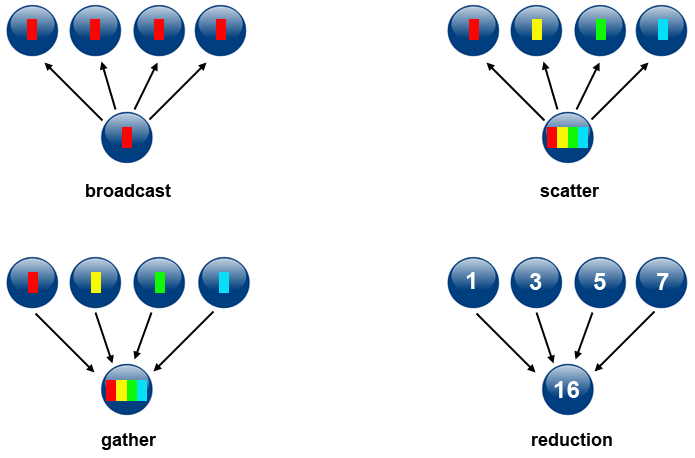
\includegraphics[width=0.5\textwidth]{../slides/image/parprog/collective_comm}
    }
  \end{block}
\end{frame}

\begin{frame}[fragile,allowframebreaks]{Collective Communication Functions}
  \begin{itemize}
    \item \bflub{MPI\_Barrier}: Creates a barrier synchronization in a group
    \item \bflub{MPI\_Bcast}: Broadcasts (sends) a message from the process with rank “root” to all other processes in the group
    \item \bflub{MPI\_Scatter}: Distributes distinct messages from a single source task to each task in the group
    \item \bflub{MPI\_Gather}: Gathers distinct messages from each task in the group to a single destination task
    \item \bflub{MPI\_Allgather}: Concatenation of data to all tasks in a group. Each task in the group, in effect, performs a one-to-all broadcasting operation within the group
    \item \bflub{MPI\_Reduce}: Applies a reduction operation on all tasks in the group and places the result in one task
    \item \bflub{MPI\_Allreduce}: equivalent to an \lstC{MPI\_Reduce} followed by an \lstC{MPI\_Bcast}
    \item \bflub{MPI\_Reduce\_scatter} equivalent to an \lstC{MPI\_Reduce} followed by an \lstC{MPI\_Scatter operation}
    \item \bflub{MPI\_Alltoall}: Each task in a group performs a scatter operation, sending a distinct message to all the tasks in the group in order by index
    \item \bflub{MPI\_Scan}: Performs a scan operation with respect to a reduction operation across a task group
  \end{itemize}
  \framebreak
  \begin{block}{}
  \begin{lstlisting}[basicstyle=\scriptsize\ttfamily,language=C]
MPI_Bcast (&buffer,count,datatype,root,comm)
MPI_Scatter (&sendbuf,sendcnt,sendtype,&recvbuf,recvcnt,recvtype,root,comm)
MPI_Gather (&sendbuf,sendcnt,sendtype,&recvbuf,recvcount,recvtype,root,comm)
MPI_Allgather (&sendbuf,sendcount,sendtype,&recvbuf,recvcount,recvtype,comm)
MPI_Reduce (&sendbuf,&recvbuf,count,datatype,op,root,comm)
MPI_Allreduce (&sendbuf,&recvbuf,count,datatype,op,comm)
MPI_Reduce_scatter (&sendbuf,&recvbuf,recvcount,datatype,op,comm)
MPI_Alltoall (&sendbuf,sendcount,sendtype,&recvbuf,recvcnt,recvtype,comm)
MPI_Scan (&sendbuf,&recvbuf,count,datatype,op,comm)
  \end{lstlisting}
  \begin{lstlisting}[basicstyle=\scriptsize\ttfamily,language=Fortran]
MPI_BCAST (buffer,count,datatype,root,comm,ierr)
MPI_SCATTER (sendbuf,sendcnt,sendtype,recvbuf,recvcnt,recvtype,root,comm,ierr)MPI_GATHER (sendbuf,sendcnt,sendtype,recvbuf,recvcount,recvtype,root,comm,ierr)
MPI_ALLGATHER (sendbuf,sendcount,sendtype,recvbuf,recvcount,recvtype,comm,info)
MPI_REDUCE (sendbuf,recvbuf,count,datatype,op,root,comm,ierr)
MPI_ALLREDUCE (sendbuf,recvbuf,count,datatype,op,comm,ierr)
MPI_REDUCE_SCATTER (sendbuf,recvbuf,recvcount,datatype,op,comm,ierr)
MPI_ALLTOALL (sendbuf,sendcount,sendtype,recvbuf,recvcnt,recvtype,comm,ierr)
MPI_SCAN (sendbuf,recvbuf,count,datatype,op,comm,ierr)
  \end{lstlisting}
  \end{block}
\end{frame}

\begin{frame}[fragile,allowframebreaks]{Exercise: Calculation of Pi}
  \begin{itemize}
    \item Parallelize the \lstC{pi_mpi.f90} or \lstC{pi_mpi.c} making use of collective communication functions?
  \end{itemize}
  \begin{exampleblock}{}
    \begin{lstlisting}[basicstyle=\scriptsize\ttfamily]
[alp514.sol](1061): mpicc -o pic pi_mpi.c
[alp514.sol](1062): mpif90 -o pif pi_mpi.f90
[alp514.sol](1063): srun -n 6 -p hawkgpu --reservation=lts_165 -t 10 ./pic
pi = 3.141592653589771
time to compute = 0.02951 seconds

[alp514.sol](1064): srun -n 6 -p hawkgpu --reservation=lts_165 -t 10 ./pif
pi = 3.141592633589724
time to compute =    0.023 seconds

[alp514.sol](1065): srun -N 2 --ntasks-per-node=3 -p infolab -t 10  ./pic
pi = 3.141592653589771
time to compute = 0.0282662 seconds

[alp514.sol](1066): srun -N 2 --ntasks-per-node=3 -p infolab -t 10  ./pif
pi = 3.141592633589724
time to compute =    0.015 seconds
    \end{lstlisting}
  \end{exampleblock}
  \framebreak
  \begin{exampleblock}{}
    \begin{lstlisting}[basicstyle=\scriptsize\ttfamily]
[alp514.sol](1081): srun -N 2 --ntasks-per-node=12 -p chem -t 10  ./pic
pi = 3.141592653589797
time to compute = 0.014163 seconds

[alp514.sol](1082): srun -N 2 --ntasks-per-node=12 -p chem -t 10  ./pif
pi = 3.141592633589827
time to compute =    0.007 seconds

[alp514.sol](1083): srun -N 2 --ntasks-per-node=24 -p chem -t 10  ./pic
pi = 3.141592653589789
time to compute = 0.0264809 seconds

[alp514.sol](1084): srun -N 2 --ntasks-per-node=24 -p chem -t 10  ./pif
pi = 3.141592633589773
time to compute =    0.038 seconds

[alp514.sol](1085): srun -N 2 --ntasks-per-node=36 -p chem -t 10  ./pic
pi = 3.141592653589792
time to compute = 0.184978 seconds

[alp514.sol](1086): srun -N 2 --ntasks-per-node=36 -p chem -t 10  ./pif
pi = 3.141592633589787
time to compute =    0.014 seconds
    \end{lstlisting}
  \end{exampleblock}
\end{frame}



\begin{frame}{Further Reading}
  \begin{itemize}
    \item Books
    \begin{enumerate}
      \item Parallel Programming with MPI by Peter Pacheco (No relation)
      \item Using MPI - 2nd Edition: Portable Parallel Programming with the Message Passing Interface (Scientific and Engineering Computation) by William Gropp
      \item Parallel Programming in C with MPI and Openmp by Michael J. Quinn
      \item MPI: The Complete Reference by Marc Snir \textit{et. al.}
      \item Beginning MPI (An Introduction in C) by Wesley Kendall      
      \item[] Online version: \url{http://mpitutorial.com/}
    \end{enumerate}
    \item Tutorials
    \begin{enumerate}
      \item MPI: \url{https://computing.llnl.gov/tutorials/mpi/}
      \item Advanced MPI: \url{https://hpc.llnl.gov/sites/default/files/DavidCronkSlides.pdf}
      \item \url{https://www.hpc-training.org/xsede/moodle}
      \item XSEDE HPC Monthly Workshop Series: \url{https://psc.edu/xsede-hpc-series-all-workshops}
    \end{enumerate}
  \end{itemize}
\end{frame}

\end{document}

